\documentclass{standalone}

\usepackage{tikz}
\usetikzlibrary{automata, positioning}

\begin{document}
    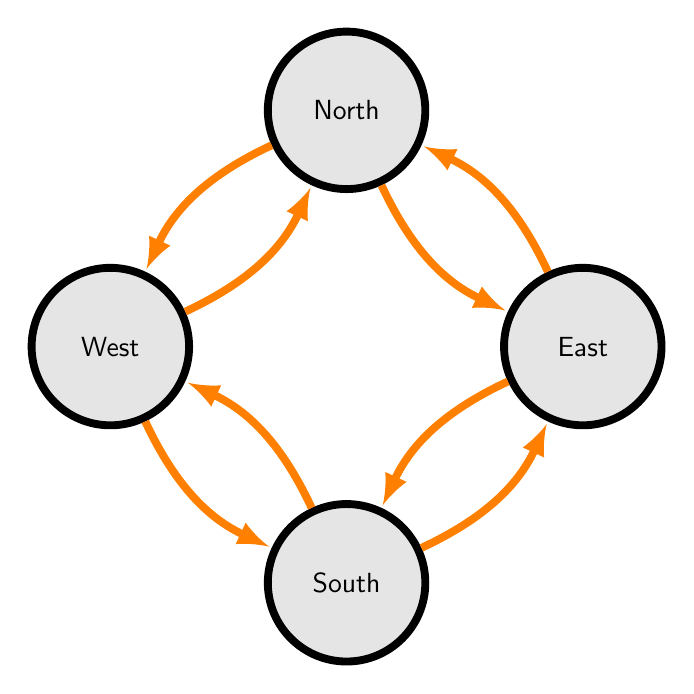
\begin{tikzpicture}[font=\sffamily]

        % Setup the style for the states
        \tikzset{node style/.style={state, 
                                    minimum width=2cm,
                                    line width=1mm,
                                    fill=gray!20!white}}

        % Draw the states
        \node[node style] at (0, 0)      (S)     {South};
        \node[node style] at (3, 3)      (E)     {East};
        \node[node style] at (0, 6)      (N)     {North};
        \node[node style] at (-3, 3)     (W)     {West};

        % Connect the states with arrows
        \draw[every loop,
              auto=right,
              line width=1mm,
              >=latex,
              draw=orange,
              fill=orange]
        (S)     edge[bend right=20]            node {} (E)
        (E)     edge[bend right=20]            node {} (S)
        (E)     edge[bend right=20]            node {} (N)
        (N)     edge[bend right=20]            node {} (E)
        (N)     edge[bend right=20]            node {} (W)
        (W)     edge[bend right=20]            node {} (N)
        (W)     edge[bend right=20]            node {} (S)
        (S)     edge[bend right=20]            node {} (W);
    \end{tikzpicture}
\end{document}